\documentclass[a3paper,landscape]{article}
\usepackage[a3paper,landscape,margin=1cm]{geometry}
\usepackage{tikz}
\usepackage{xcolor}
\usepackage[T1]{fontenc}
\usepackage[utf8]{inputenc}
\usepackage{lmodern}
\usetikzlibrary{shapes.geometric, arrows.meta, positioning, fit, backgrounds, calc, shadows}

\definecolor{stageblue}{RGB}{30,80,160}
\definecolor{pastelblue}{RGB}{173,216,230}
\definecolor{pastelpink}{RGB}{255,182,193}
\definecolor{pastelgreen}{RGB}{144,238,144}
\definecolor{pastelyellow}{RGB}{255,255,153}
\definecolor{pastellavender}{RGB}{216,191,216}
\definecolor{pastelcyan}{RGB}{175,238,238}

\begin{document}
\pagestyle{empty}
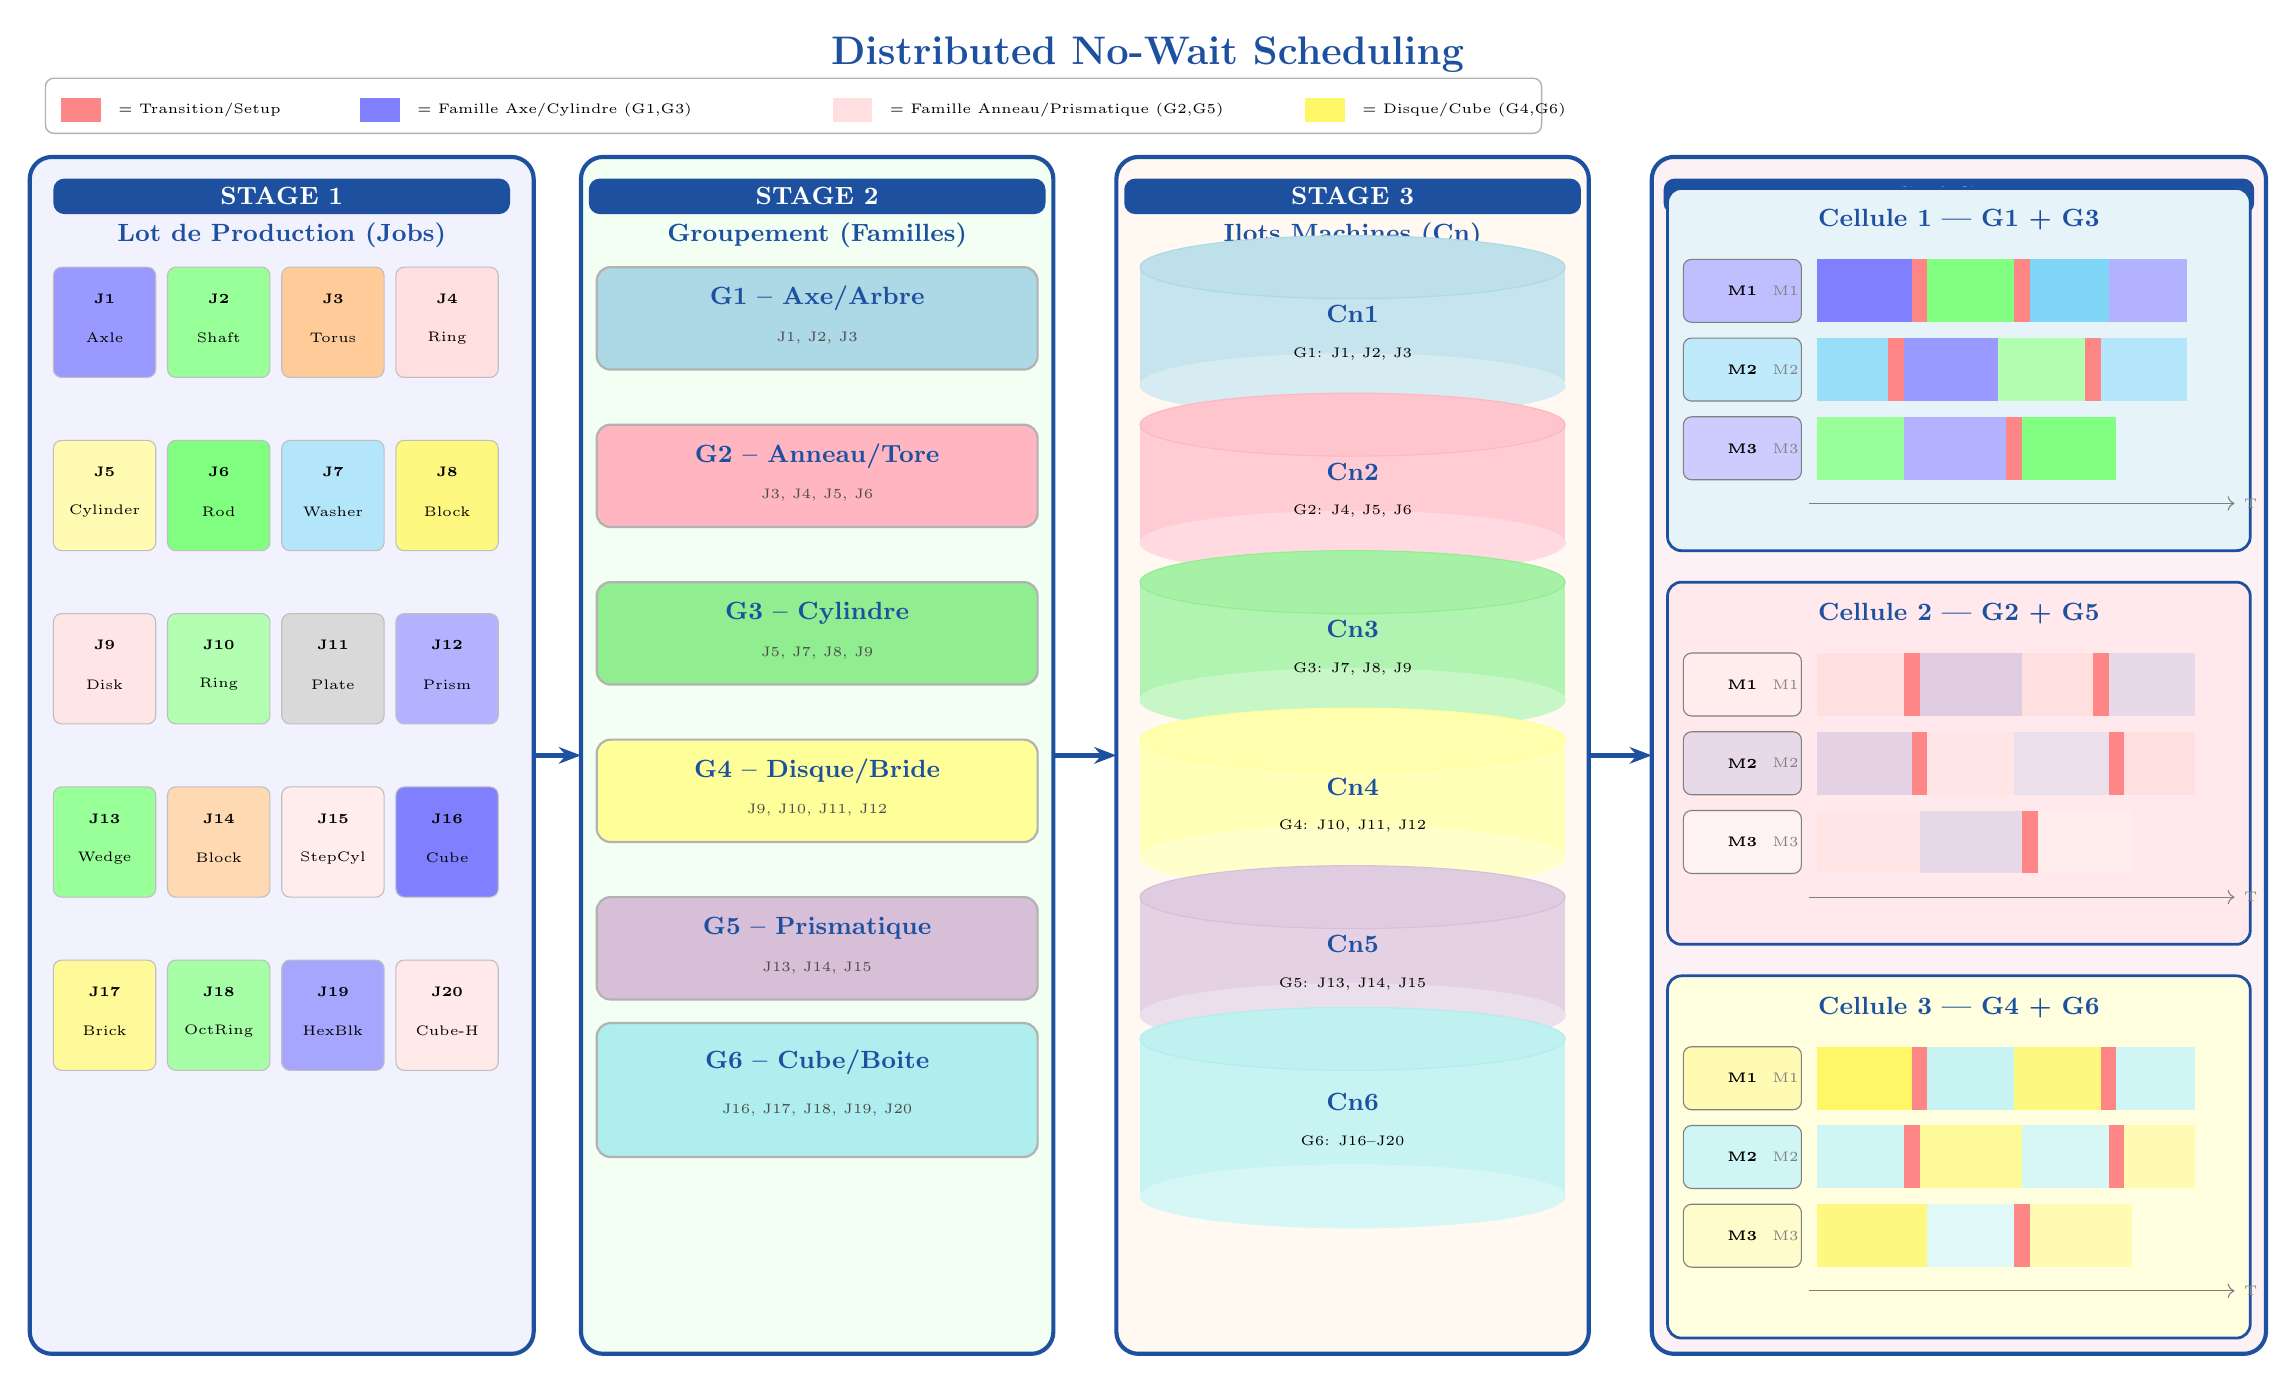
\begin{tikzpicture}[font=\sffamily]

%% TITLE
\node[align=center, font=\bfseries\Large, text=stageblue] at (14,16.5)
  {\textbf{Distributed No-Wait Scheduling}};
\node[align=center, font=\small, text=gray] at (14,15.9)
  {Infographie technique --- Ordonnancement distribue sans attente};

%% STAGE BOXES
\draw[rounded corners=8pt, fill=blue!5, draw=stageblue, line width=1.5pt]
  (-0.2,0) rectangle (6.2,15.2);
\node[fill=stageblue, text=white, rounded corners=4pt, font=\bfseries\small,
  minimum width=5.8cm, align=center] at (3,14.7) {STAGE 1};
\node[font=\bfseries\small, text=stageblue, align=center] at (3,14.2)
  {Lot de Production (Jobs)};

\draw[rounded corners=8pt, fill=green!5, draw=stageblue, line width=1.5pt]
  (6.8,0) rectangle (12.8,15.2);
\node[fill=stageblue, text=white, rounded corners=4pt, font=\bfseries\small,
  minimum width=5.8cm, align=center] at (9.8,14.7) {STAGE 2};
\node[font=\bfseries\small, text=stageblue, align=center] at (9.8,14.2)
  {Groupement (Familles)};

\draw[rounded corners=8pt, fill=orange!5, draw=stageblue, line width=1.5pt]
  (13.6,0) rectangle (19.6,15.2);
\node[fill=stageblue, text=white, rounded corners=4pt, font=\bfseries\small,
  minimum width=5.8cm, align=center] at (16.6,14.7) {STAGE 3};
\node[font=\bfseries\small, text=stageblue, align=center] at (16.6,14.2)
  {Ilots Machines (Cn)};

\draw[rounded corners=8pt, fill=purple!5, draw=stageblue, line width=1.5pt]
  (20.4,0) rectangle (28.2,15.2);
\node[fill=stageblue, text=white, rounded corners=4pt, font=\bfseries\small,
  minimum width=7.5cm, align=center] at (24.3,14.7) {STAGE 4};
\node[font=\bfseries\small, text=stageblue, align=center] at (24.3,14.2)
  {Fabrication + Diagramme de Gantt};

%% ARROWS
\draw[-{Stealth[length=8pt]}, line width=2pt, color=stageblue]
  (6.2,7.6) -- (6.8,7.6);
\draw[-{Stealth[length=8pt]}, line width=2pt, color=stageblue]
  (12.8,7.6) -- (13.6,7.6);
\draw[-{Stealth[length=8pt]}, line width=2pt, color=stageblue]
  (19.6,7.6) -- (20.4,7.6);

%% STAGE 1: JOB CARDS
\draw[rounded corners=3pt,fill=blue!40,draw=gray!50] (0.1,12.4) rectangle (1.4,13.8);
\node[font=\bfseries\tiny] at (0.75,13.4) {J1}; \node[font=\tiny] at (0.75,12.9) {Axle};
\draw[rounded corners=3pt,fill=green!40,draw=gray!50] (1.55,12.4) rectangle (2.85,13.8);
\node[font=\bfseries\tiny] at (2.2,13.4) {J2}; \node[font=\tiny] at (2.2,12.9) {Shaft};
\draw[rounded corners=3pt,fill=orange!40,draw=gray!50] (3.0,12.4) rectangle (4.3,13.8);
\node[font=\bfseries\tiny] at (3.65,13.4) {J3}; \node[font=\tiny] at (3.65,12.9) {Torus};
\draw[rounded corners=3pt,fill=pink!50,draw=gray!50] (4.45,12.4) rectangle (5.75,13.8);
\node[font=\bfseries\tiny] at (5.1,13.4) {J4}; \node[font=\tiny] at (5.1,12.9) {Ring};
\draw[rounded corners=3pt,fill=yellow!30,draw=gray!50] (0.1,10.2) rectangle (1.4,11.6);
\node[font=\bfseries\tiny] at (0.75,11.2) {J5}; \node[font=\tiny] at (0.75,10.7) {Cylinder};
\draw[rounded corners=3pt,fill=green!50,draw=gray!50] (1.55,10.2) rectangle (2.85,11.6);
\node[font=\bfseries\tiny] at (2.2,11.2) {J6}; \node[font=\tiny] at (2.2,10.7) {Rod};
\draw[rounded corners=3pt,fill=cyan!30,draw=gray!50] (3.0,10.2) rectangle (4.3,11.6);
\node[font=\bfseries\tiny] at (3.65,11.2) {J7}; \node[font=\tiny] at (3.65,10.7) {Washer};
\draw[rounded corners=3pt,fill=yellow!50,draw=gray!50] (4.45,10.2) rectangle (5.75,11.6);
\node[font=\bfseries\tiny] at (5.1,11.2) {J8}; \node[font=\tiny] at (5.1,10.7) {Block};
\draw[rounded corners=3pt,fill=pink!40,draw=gray!50] (0.1,8.0) rectangle (1.4,9.4);
\node[font=\bfseries\tiny] at (0.75,9.0) {J9}; \node[font=\tiny] at (0.75,8.5) {Disk};
\draw[rounded corners=3pt,fill=green!30,draw=gray!50] (1.55,8.0) rectangle (2.85,9.4);
\node[font=\bfseries\tiny] at (2.2,9.0) {J10}; \node[font=\tiny] at (2.2,8.5) {Ring};
\draw[rounded corners=3pt,fill=gray!30,draw=gray!50] (3.0,8.0) rectangle (4.3,9.4);
\node[font=\bfseries\tiny] at (3.65,9.0) {J11}; \node[font=\tiny] at (3.65,8.5) {Plate};
\draw[rounded corners=3pt,fill=blue!30,draw=gray!50] (4.45,8.0) rectangle (5.75,9.4);
\node[font=\bfseries\tiny] at (5.1,9.0) {J12}; \node[font=\tiny] at (5.1,8.5) {Prism};
\draw[rounded corners=3pt,fill=green!40,draw=gray!50] (0.1,5.8) rectangle (1.4,7.2);
\node[font=\bfseries\tiny] at (0.75,6.8) {J13}; \node[font=\tiny] at (0.75,6.3) {Wedge};
\draw[rounded corners=3pt,fill=orange!30,draw=gray!50] (1.55,5.8) rectangle (2.85,7.2);
\node[font=\bfseries\tiny] at (2.2,6.8) {J14}; \node[font=\tiny] at (2.2,6.3) {Block};
\draw[rounded corners=3pt,fill=pink!30,draw=gray!50] (3.0,5.8) rectangle (4.3,7.2);
\node[font=\bfseries\tiny] at (3.65,6.8) {J15}; \node[font=\tiny] at (3.65,6.3) {StepCyl};
\draw[rounded corners=3pt,fill=blue!50,draw=gray!50] (4.45,5.8) rectangle (5.75,7.2);
\node[font=\bfseries\tiny] at (5.1,6.8) {J16}; \node[font=\tiny] at (5.1,6.3) {Cube};
\draw[rounded corners=3pt,fill=yellow!40,draw=gray!50] (0.1,3.6) rectangle (1.4,5.0);
\node[font=\bfseries\tiny] at (0.75,4.6) {J17}; \node[font=\tiny] at (0.75,4.1) {Brick};
\draw[rounded corners=3pt,fill=green!35,draw=gray!50] (1.55,3.6) rectangle (2.85,5.0);
\node[font=\bfseries\tiny] at (2.2,4.6) {J18}; \node[font=\tiny] at (2.2,4.1) {OctRing};
\draw[rounded corners=3pt,fill=blue!35,draw=gray!50] (3.0,3.6) rectangle (4.3,5.0);
\node[font=\bfseries\tiny] at (3.65,4.6) {J19}; \node[font=\tiny] at (3.65,4.1) {HexBlk};
\draw[rounded corners=3pt,fill=pink!35,draw=gray!50] (4.45,3.6) rectangle (5.75,5.0);
\node[font=\bfseries\tiny] at (5.1,4.6) {J20}; \node[font=\tiny] at (5.1,4.1) {Cube-H};

%% STAGE 2: GROUP CARDS
\draw[rounded corners=5pt,fill=pastelblue,draw=gray!60,line width=0.8pt]
  (7.0,12.5) rectangle (12.6,13.8);
\node[font=\bfseries\small,text=stageblue] at (9.8,13.4) {G1 -- Axe/Arbre};
\node[font=\tiny,text=black!70] at (9.8,12.9) {J1, J2, J3};

\draw[rounded corners=5pt,fill=pastelpink,draw=gray!60,line width=0.8pt]
  (7.0,10.5) rectangle (12.6,11.8);
\node[font=\bfseries\small,text=stageblue] at (9.8,11.4) {G2 -- Anneau/Tore};
\node[font=\tiny,text=black!70] at (9.8,10.9) {J3, J4, J5, J6};

\draw[rounded corners=5pt,fill=pastelgreen,draw=gray!60,line width=0.8pt]
  (7.0,8.5) rectangle (12.6,9.8);
\node[font=\bfseries\small,text=stageblue] at (9.8,9.4) {G3 -- Cylindre};
\node[font=\tiny,text=black!70] at (9.8,8.9) {J5, J7, J8, J9};

\draw[rounded corners=5pt,fill=pastelyellow,draw=gray!60,line width=0.8pt]
  (7.0,6.5) rectangle (12.6,7.8);
\node[font=\bfseries\small,text=stageblue] at (9.8,7.4) {G4 -- Disque/Bride};
\node[font=\tiny,text=black!70] at (9.8,6.9) {J9, J10, J11, J12};

\draw[rounded corners=5pt,fill=pastellavender,draw=gray!60,line width=0.8pt]
  (7.0,4.5) rectangle (12.6,5.8);
\node[font=\bfseries\small,text=stageblue] at (9.8,5.4) {G5 -- Prismatique};
\node[font=\tiny,text=black!70] at (9.8,4.9) {J13, J14, J15};

\draw[rounded corners=5pt,fill=pastelcyan,draw=gray!60,line width=0.8pt]
  (7.0,2.5) rectangle (12.6,4.2);
\node[font=\bfseries\small,text=stageblue] at (9.8,3.7) {G6 -- Cube/Boite};
\node[font=\tiny,text=black!70] at (9.8,3.1) {J16, J17, J18, J19, J20};

%% STAGE 3: CYLINDERS
\fill[pastelblue!70] (13.9,12.3) rectangle (19.3,13.8);
\draw[pastelblue,fill=pastelblue!80] (16.6,13.8) ellipse (2.7 and 0.4);
\draw[pastelblue!50,fill=pastelblue!50] (16.6,12.3) ellipse (2.7 and 0.4);
\node[font=\bfseries\small,text=stageblue] at (16.6,13.2) {Cn1};
\node[font=\tiny] at (16.6,12.7) {G1: J1, J2, J3};

\fill[pastelpink!70] (13.9,10.3) rectangle (19.3,11.8);
\draw[pastelpink,fill=pastelpink!80] (16.6,11.8) ellipse (2.7 and 0.4);
\draw[pastelpink!50,fill=pastelpink!50] (16.6,10.3) ellipse (2.7 and 0.4);
\node[font=\bfseries\small,text=stageblue] at (16.6,11.2) {Cn2};
\node[font=\tiny] at (16.6,10.7) {G2: J4, J5, J6};

\fill[pastelgreen!70] (13.9,8.3) rectangle (19.3,9.8);
\draw[pastelgreen,fill=pastelgreen!80] (16.6,9.8) ellipse (2.7 and 0.4);
\draw[pastelgreen!50,fill=pastelgreen!50] (16.6,8.3) ellipse (2.7 and 0.4);
\node[font=\bfseries\small,text=stageblue] at (16.6,9.2) {Cn3};
\node[font=\tiny] at (16.6,8.7) {G3: J7, J8, J9};

\fill[pastelyellow!70] (13.9,6.3) rectangle (19.3,7.8);
\draw[pastelyellow,fill=pastelyellow!80] (16.6,7.8) ellipse (2.7 and 0.4);
\draw[pastelyellow!50,fill=pastelyellow!50] (16.6,6.3) ellipse (2.7 and 0.4);
\node[font=\bfseries\small,text=stageblue] at (16.6,7.2) {Cn4};
\node[font=\tiny] at (16.6,6.7) {G4: J10, J11, J12};

\fill[pastellavender!70] (13.9,4.3) rectangle (19.3,5.8);
\draw[pastellavender,fill=pastellavender!80] (16.6,5.8) ellipse (2.7 and 0.4);
\draw[pastellavender!50,fill=pastellavender!50] (16.6,4.3) ellipse (2.7 and 0.4);
\node[font=\bfseries\small,text=stageblue] at (16.6,5.2) {Cn5};
\node[font=\tiny] at (16.6,4.7) {G5: J13, J14, J15};

\fill[pastelcyan!70] (13.9,2.0) rectangle (19.3,4.0);
\draw[pastelcyan,fill=pastelcyan!80] (16.6,4.0) ellipse (2.7 and 0.4);
\draw[pastelcyan!50,fill=pastelcyan!50] (16.6,2.0) ellipse (2.7 and 0.4);
\node[font=\bfseries\small,text=stageblue] at (16.6,3.2) {Cn6};
\node[font=\tiny] at (16.6,2.7) {G6: J16--J20};

%% STAGE 4: CELL 1
\draw[rounded corners=5pt,fill=pastelblue!30,draw=stageblue,line width=1pt]
  (20.6,10.2) rectangle (28.0,14.8);
\node[font=\bfseries\small,text=stageblue] at (24.3,14.4) {Cellule 1 --- G1 + G3};
\draw[fill=blue!25,rounded corners=3pt,draw=gray] (20.8,13.1) rectangle (22.3,13.9);
\node[font=\tiny\bfseries] at (21.55,13.5) {M1};
\draw[fill=cyan!25,rounded corners=3pt,draw=gray] (20.8,12.1) rectangle (22.3,12.9);
\node[font=\tiny\bfseries] at (21.55,12.5) {M2};
\draw[fill=blue!20,rounded corners=3pt,draw=gray] (20.8,11.1) rectangle (22.3,11.9);
\node[font=\tiny\bfseries] at (21.55,11.5) {M3};
\fill[blue!50] (22.5,13.1) rectangle (23.7,13.9);
\fill[pink!70!red] (23.7,13.1) rectangle (23.9,13.9);
\fill[green!50] (23.9,13.1) rectangle (25.0,13.9);
\fill[pink!70!red] (25.0,13.1) rectangle (25.2,13.9);
\fill[cyan!50] (25.2,13.1) rectangle (26.2,13.9);
\fill[blue!30] (26.2,13.1) rectangle (27.2,13.9);
\fill[cyan!40] (22.5,12.1) rectangle (23.4,12.9);
\fill[pink!70!red] (23.4,12.1) rectangle (23.6,12.9);
\fill[blue!40] (23.6,12.1) rectangle (24.8,12.9);
\fill[green!30] (24.8,12.1) rectangle (25.9,12.9);
\fill[pink!70!red] (25.9,12.1) rectangle (26.1,12.9);
\fill[cyan!30] (26.1,12.1) rectangle (27.2,12.9);
\fill[green!40] (22.5,11.1) rectangle (23.6,11.9);
\fill[blue!30] (23.6,11.1) rectangle (24.9,11.9);
\fill[pink!70!red] (24.9,11.1) rectangle (25.1,11.9);
\fill[green!50] (25.1,11.1) rectangle (26.3,11.9);
\draw[->,gray,thin] (22.4,10.8) -- (27.8,10.8) node[right,font=\tiny]{T};
\node[font=\tiny,gray] at (22.1,13.5) {M1};
\node[font=\tiny,gray] at (22.1,12.5) {M2};
\node[font=\tiny,gray] at (22.1,11.5) {M3};

%% STAGE 4: CELL 2
\draw[rounded corners=5pt,fill=pastelpink!30,draw=stageblue,line width=1pt]
  (20.6,5.2) rectangle (28.0,9.8);
\node[font=\bfseries\small,text=stageblue] at (24.3,9.4) {Cellule 2 --- G2 + G5};
\draw[fill=pink!30,rounded corners=3pt,draw=gray] (20.8,8.1) rectangle (22.3,8.9);
\node[font=\tiny\bfseries] at (21.55,8.5) {M1};
\draw[fill=pastellavender!60,rounded corners=3pt,draw=gray] (20.8,7.1) rectangle (22.3,7.9);
\node[font=\tiny\bfseries] at (21.55,7.5) {M2};
\draw[fill=pink!20,rounded corners=3pt,draw=gray] (20.8,6.1) rectangle (22.3,6.9);
\node[font=\tiny\bfseries] at (21.55,6.5) {M3};
\fill[pink!50] (22.5,8.1) rectangle (23.6,8.9);
\fill[pink!70!red] (23.6,8.1) rectangle (23.8,8.9);
\fill[pastellavender!80] (23.8,8.1) rectangle (25.1,8.9);
\fill[pink!50] (25.1,8.1) rectangle (26.0,8.9);
\fill[pink!70!red] (26.0,8.1) rectangle (26.2,8.9);
\fill[pastellavender!60] (26.2,8.1) rectangle (27.3,8.9);
\fill[pastellavender!70] (22.5,7.1) rectangle (23.7,7.9);
\fill[pink!70!red] (23.7,7.1) rectangle (23.9,7.9);
\fill[pink!40] (23.9,7.1) rectangle (25.0,7.9);
\fill[pastellavender!50] (25.0,7.1) rectangle (26.2,7.9);
\fill[pink!70!red] (26.2,7.1) rectangle (26.4,7.9);
\fill[pink!50] (26.4,7.1) rectangle (27.3,7.9);
\fill[pink!40] (22.5,6.1) rectangle (23.8,6.9);
\fill[pastellavender!60] (23.8,6.1) rectangle (25.1,6.9);
\fill[pink!70!red] (25.1,6.1) rectangle (25.3,6.9);
\fill[pink!30] (25.3,6.1) rectangle (26.5,6.9);
\draw[->,gray,thin] (22.4,5.8) -- (27.8,5.8) node[right,font=\tiny]{T};
\node[font=\tiny,gray] at (22.1,8.5) {M1};
\node[font=\tiny,gray] at (22.1,7.5) {M2};
\node[font=\tiny,gray] at (22.1,6.5) {M3};

%% STAGE 4: CELL 3
\draw[rounded corners=5pt,fill=pastelyellow!30,draw=stageblue,line width=1pt]
  (20.6,0.2) rectangle (28.0,4.8);
\node[font=\bfseries\small,text=stageblue] at (24.3,4.4) {Cellule 3 --- G4 + G6};
\draw[fill=yellow!30,rounded corners=3pt,draw=gray] (20.8,3.1) rectangle (22.3,3.9);
\node[font=\tiny\bfseries] at (21.55,3.5) {M1};
\draw[fill=pastelcyan!60,rounded corners=3pt,draw=gray] (20.8,2.1) rectangle (22.3,2.9);
\node[font=\tiny\bfseries] at (21.55,2.5) {M2};
\draw[fill=yellow!20,rounded corners=3pt,draw=gray] (20.8,1.1) rectangle (22.3,1.9);
\node[font=\tiny\bfseries] at (21.55,1.5) {M3};
\fill[yellow!60] (22.5,3.1) rectangle (23.7,3.9);
\fill[pink!70!red] (23.7,3.1) rectangle (23.9,3.9);
\fill[pastelcyan!70] (23.9,3.1) rectangle (25.0,3.9);
\fill[yellow!50] (25.0,3.1) rectangle (26.1,3.9);
\fill[pink!70!red] (26.1,3.1) rectangle (26.3,3.9);
\fill[pastelcyan!60] (26.3,3.1) rectangle (27.3,3.9);
\fill[pastelcyan!60] (22.5,2.1) rectangle (23.6,2.9);
\fill[pink!70!red] (23.6,2.1) rectangle (23.8,2.9);
\fill[yellow!40] (23.8,2.1) rectangle (25.1,2.9);
\fill[pastelcyan!50] (25.1,2.1) rectangle (26.2,2.9);
\fill[pink!70!red] (26.2,2.1) rectangle (26.4,2.9);
\fill[yellow!30] (26.4,2.1) rectangle (27.3,2.9);
\fill[yellow!50] (22.5,1.1) rectangle (23.9,1.9);
\fill[pastelcyan!40] (23.9,1.1) rectangle (25.0,1.9);
\fill[pink!70!red] (25.0,1.1) rectangle (25.2,1.9);
\fill[yellow!30] (25.2,1.1) rectangle (26.5,1.9);
\draw[->,gray,thin] (22.4,0.8) -- (27.8,0.8) node[right,font=\tiny]{T};
\node[font=\tiny,gray] at (22.1,3.5) {M1};
\node[font=\tiny,gray] at (22.1,2.5) {M2};
\node[font=\tiny,gray] at (22.1,1.5) {M3};

%% LEGEND
\draw[rounded corners=3pt,fill=white,draw=gray!60,line width=0.5pt]
  (0.0,15.5) rectangle (19.0,16.2);
\fill[pink!70!red] (0.2,15.65) rectangle (0.7,15.95);
\node[font=\tiny,right] at (0.8,15.8) {= Transition/Setup};
\fill[blue!50] (4.0,15.65) rectangle (4.5,15.95);
\node[font=\tiny,right] at (4.6,15.8) {= Famille Axe/Cylindre (G1,G3)};
\fill[pink!50] (10.0,15.65) rectangle (10.5,15.95);
\node[font=\tiny,right] at (10.6,15.8) {= Famille Anneau/Prismatique (G2,G5)};
\fill[yellow!60] (16.0,15.65) rectangle (16.5,15.95);
\node[font=\tiny,right] at (16.6,15.8) {= Disque/Cube (G4,G6)};

\end{tikzpicture}
\end{document}
